\chapter{Genetralized Linear Model (GLM) (COMING SOON)}
\label{ch-gen-lin-mod}

This chapter is based on
chapter 4 of Ref.\cite{agresti-book}.

\section{Exponential Family of Distributions}
\label{sec-exp-fam}

Exponential Family (EF) of distributions

\beq
P(y|\theta, \phi) =
\exp\left(\frac{\theta y - b(\theta)}{a(\phi)}+c(y,\phi)\right)
\eeq


\begin{claim}
\beq
\mu = E[\rvy] = b'(\theta)
\eeq

\beq
\s^2= \av{\rvy, \rvy} = a(\phi)b''(\theta)
\eeq
\end{claim}
\proof

\beqa
0&=& \partial_\theta \int_{-\infty}^\infty
dy\; P(y|\theta, \phi)
\\
&=&
\int_{-\infty}^\infty
dy\;\frac{1}{a}
[y-b'(\theta)]P(y|\theta, \phi)
\\
&=&
\frac{1}{a}[E[\rvy]-b'(\theta)]
\eeqa

\beqa
0&=& \partial^2_\theta \int_{-\infty}^\infty
dy\; P(y|\theta, \phi)
\\
&=&
\int_{-\infty}^\infty
dy\;\left\{\frac{-b''(\theta)}{a} +
\frac{1}{a^2}
[y-b'(\theta)]^2\right\}
P(y|\theta, \phi)
\eeqa
Hence,

\beq
\av{[y-b'(\theta)]^2}= a b''(\theta)
\eeq

\qed

\beqa
\caln(y; \mu, \s^2)
&=&
\frac{1}{\sqrt{2\pi \s^2}}
\exp\left(
-\frac{(y-\mu)^2}{2\s^2}
\right)
\\
&=&
\exp\left(
\frac{-y^2 + 2\mu y -\mu^2}{2\s^2}
-\ln\sqrt{2\pi \s^2}
\right)
\\
&=&
\exp\left(
\frac{-\frac{1}{2}y^2 + \mu y -\frac{1}{2}\mu^2}{\s^2}
-\ln\sqrt{2\pi \s^2}
\right)
\eeqa
So, for the
Normal Distribution, $\theta=\mu$ , $a=\s^2$, $b=\mu^2/2$,
$b'=\mu$, $b''=1$.

\beq
P(\vecy|\vtheta, \phi) =
\prod_\s
\exp\left(\frac{\theta_\s y_\s - b(\theta_\s)}{a(\phi)}+c(y_\s ,\phi)\right)
\eeq

\beq
\mu_\s = E[\rvy_\s]= \partial_{\theta_\s} b
\eeq

\beq
\av{\rvy_\s, \rvy_{\s'}} =
\delta(\s, \s')
 a\partial_{\theta_\s}\partial_{\theta_{\s'}}b
\eeq

\section{GLM}
The Generalized Linear Model (GLM)
is a way of modelling a random variable $\rvy_\s$.
A GML
has 3 parts:

\begin{enumerate}
\item Exponential Family

Model $\rvy_\s$ by probability distribution
of exponential family (EF).
EF is described in Section [\nameref{sec-exp-fam}]]

\item Linear predictor

In EF, replace $\theta_\s$
the {\bf linear predictor} $\xbeta= \sum_i X_{\s, i}\beta_i$.
$\xbeta$ is commonly denoted by $\eta_\s$,
but I will avoid that convention because
I think results are much clearer
if one uses the more explicit $\xbeta$ instead.

\item Link Function

\beq
\mu_\s = E[\rvy_\s] = \partial_{\xbeta} b
\eeq

\beq
\xbeta = g(\mu_\s) = \hat{\theta}(\mu_\s)
\eeq

\beq
\mu_\s = g^{-1}(\xbeta)=\hat{\mu}(\xbeta)
\eeq


$\hat{\theta}()=g()$ is called
the {\bf link function}.
\end{enumerate}


For Linear Regression, $\mu_\s = \xbeta$,
so the link function and its
inverse are the identity map.

\beqa
Ber(y_\s;p_\s) &=& p_\s^{y_\s} (1-p_\s)^{1-y_\s}
\\
&=&
\exp(y_\s\ln p_\s + (1-y_\s)\ln(1-p_\s))
\\
&=&
\exp\left( y_\s
\underbrace{\ln\left(\frac{p_\s}{1-p_\s}\right)}_{\xbeta}
+\underbrace{\ln (1-p_\s)}_{-b}\right)
\eeqa


$\mu_\s = p_\s$,
and $\xbeta= \lodds(\mu_\s)$ so $\mu_\s= \smoid(\xbeta)$.

$g() =\lodds()$ and $g^{-1}() =\smoid()$

\beq
a=1
\eeq

\beqa
b
&=&
 -\ln (1-\mu_\s)
\\
&=&
-\ln\left(
1- \frac{1}{1+e^{-\xbeta}}
\right)
\\
&=&
-\ln\left(
\frac{e^{-\xbeta}}{1+e^{-\xbeta}}
\right)
\\
&=&
\ln(1+e^{\xbeta})
\eeqa

\beqa
\partial_{\xbeta} b &=&
\frac{e^{\xbeta}}{1+e^{\xbeta}}
\\
&=& \smoid(\xbeta)
\\
&=&\mu_\s
\eeqa


% Please add the following required packages to your document preamble:
% \usepackage[table,xcdraw]{xcolor}
% If you use beamer only pass "xcolor=table" option, i.e. \documentclass[xcolor=table]{beamer}
\begin{table}[h!]
\centering
\begin{tabular}{|
>{\columncolor[HTML]{FFFFC7}}l |l|l|}
\hline
\cellcolor[HTML]{F6F694}prob. distribution & \cellcolor[HTML]{F6F694}link function
$\xbeta=g(\mu_\s)$ & \cellcolor[HTML]{F6F694}$\mu_\s=g^{-1}(\xbeta)$ \\ \hline
\begin{tabular}[c]{@{}l@{}}Normal\\ $\rvy_\s\in(-\infty, +\infty)$\end{tabular} & \begin{tabular}[c]{@{}l@{}}$\xbeta= \mu_\s$\\ ($g$= identity map)\end{tabular} & $\mu_\s = \xbeta$ \\ \hline
\begin{tabular}[c]{@{}l@{}}Exponential\\ $\rvy_\s\in  (0, +\infty)$\end{tabular} & $\xbeta= -\frac{1}{\mu_\s}$ & $\mu _\s= - \frac{1}{\xbeta}$ \\ \hline
\begin{tabular}[c]{@{}l@{}}Poisson\\ $\rvy_\s\in \{0,1,2, \ldots\}$\end{tabular} & $\xbeta = \ln \mu_\s$ & $\mu_\s = \exp(\xbeta)$ \\ \hline
\begin{tabular}[c]{@{}l@{}}Bernoulli\\ $\rvy_\s\in\bool$\end{tabular} & $\xbeta = \lodds(\mu_\s)$ & $\mu_\s = \smoid(\xbeta)$ \\ \hline
\end{tabular}
\caption{Various probability distributions of the EF that have simple link functions that are easy to invert.}
\label{tab-ef-link-fun}
\end{table}


\beq
y = X\beta + \eps
\eeq

\beq
\av{\eps, \eps^T}= \s^2 I_N
\eeq

Maximum Likelihood Estimate  (MLE)

\beq
\hat{\beta}=
(X^T X)^{-1} X^T y
\eeq

\beqa
\av{\hat{\beta},\hat{\beta}^T}
&=&
\av{X^T X)^{-1} X^T y, y^T X (X^T X)^{-1}}
\\
&=&
\s^2  (X^T X)^{-1}
\eeqa

Next
we will give for the GLM,
an implicit expression
(i.e., not a closed
form) for $\av{\hat{\beta}}$
and an asymptotic
expression for
$\av{\hat{\beta}, \hat{\beta}^T}$.

Will use the results of Section [\nameref{sec-ent-like-connect}]
in our proofs, where we define
the log likelihood for the
particular case we are considering now by

\beq
 LL =  \sum_\s  LL_\s
\eeq
where

\beqa
 LL_\s &=&   LL_{y_\s|\theta_\s }
\\
&=&
\frac{y_\s\theta_\s - b(\theta_\s)}{a(\phi)} + c(y_\s, \phi)
\eeqa


\begin{claim}
(Implicit expression
for $\av{\hat{\beta}}$
for GLM)

\beq
 \sum_\s \frac{[y_\s - b'(\xbeta)]}{\av{y_\s, y_\s}}
 \pder{\hat{\mu}_\s}{\xbeta}
X_{\s, \s'} =0
\eeq
for all $\s'$.
\end{claim}
\proof


\beq
\pder{ LL_{\s}}{\beta_{\s'}}
=
\pder{ LL_{\s}}{\theta_\s}\pder{\theta_\s}{\mu_\s}
\pder{\hat{\mu}_\s}{\xbeta}\pder{\xbeta}{\beta_{\s'}}
\eeq

\beq
\pder{ LL_{\s}}{\theta_\s}  =
\frac{y_\s - b'(\theta_\s)}{a(\phi)}
\eeq

\beq
\pder{\mu_\s} {\theta_\s}
=
b''(\theta_\s) = \frac{\av{y_\s, y_\s}}{a(\phi)}
\eeq

\beq
\pder{\hat{\mu}_\s}{\xbeta} =
(g^{-1})'(\xbeta)
\eeq

\beq
\pder{\xbeta}{\beta_{\s'}}= X_{\s, \s'}
\eeq

\beq
\pder{ LL_{\s}}{\beta_{\s'}}
=
\frac{[y_\s - b'(\theta_\s)]}{\av{y_\s, y_\s}}
 \pder{\hat{\mu}_\s}{\xbeta}
X_{\s, \s'}
\eeq

\beq
0= \av{\pder{ LL}{\beta_{\s'}}}  =
\sum_\s  \pder{ LL_{\s}}{\beta_{\s'}}
=
 \sum_\s \frac{[y_\s - b'(\theta_\s)]}{\av{y_\s, y_\s}}
 \pder{\hat{\mu}_\s}{\xbeta}
X_{\s, \s'}
\eeq
for all $\s'$.
 \qed


(asymptotic covariance)
\begin{claim}
(Asymptotic expression
for $\av{\hat{\beta},\hat{\beta}^T}$
for GLM)


\beq
\av{\hat{\beta},\hat{\beta}^T}
\rarrow \cali^{-1}
\eeq
where

\beq
\cali = X^T W X
\eeq
and

\beq
W_{\s, \s'} = \left[\frac{(\partial_{\xbeta} \hat{\mu} )^2 }
{\av{y_\s, y_\s} } \delta(\s, \s')\right]_{\beta=\hat{\beta}}
\eeq
$\cali$ is called the {\bf information matrix}.
 More information, less variance.
\end{claim}
\proof

\begin{align}
\av{\pder{ LL_\s}{\beta_ { \s'}}
\pder{ LL_\s}{\beta_ { \s''}} }
&=
\av{
\frac{[y_\s - b'(\xbeta)]}{\av{y_\s, y_\s}}
 \pder{\hat{\mu}_\s}{\xbeta}
X_{\s, \s'}
\frac{[y_\s - b'(\xbeta)]}{\av{y_\s, y_\s}}
 \pder{\hat{\mu}_\s}{\xbeta}
X_{\s, \s''}
}
\\
&=
 \left[\pder{\hat{\mu}_\s}{\xbeta}\right]^2
\frac{X_{\s, \s'} X_{\s, \s''}}{\av{y_\s, y_\s}}
\end{align}

\beq
\sum_{\s}
\av{\pder{ LL_{\s}}{\beta_ { \s'}}
\pder{ LL_{\s}}{\beta_ { \s''}} }
=
(X^T W X)_{\s'', \s'}
\eeq

\beq
\av{\frac{\partial^2 LL_\s}{\partial\beta_ { \s'}\partial\beta_ { \s''}} }
=
-\av{\pder{ LL_\s}{\beta_ { \s'}}
\pder{ LL_\s}{\beta_ { \s''}} }
\eeq
Summing both sides over $\s$

\beq
\av{\frac{\partial^2 LL}{\partial\beta_ { \s'}\partial\beta_ { \s''}} }
=
-(X^T W X)_{\s'', \s'}
\eeq

\beq
\av{\hat{\beta}, \hat{\beta}^T}\rarrow (X^T W X)^{-1}
\eeq

\qed

Newton-Raphson method for calculating
estimators $\hat{\beta}$

$L=\av{ LL} =\sum_\s \av{ LL_\s}$

$u^T = [\pder{L}{\beta_\s}]_{\s=0,1,2, \ldots}$

 $H= [H_{\s, \s'}]$, $H_{\s, \s'} =
\frac{\partial^2 L }{\partial\beta_\s\partial\beta_{\s'}}$ .
$H$ is called the {\bf hessian matrix}


\beq
L(\beta)
\approx
L(\beta^{(t)})
+ u^{(t)T}(\beta-\beta^{(t)})
+ \frac{1}{2}
(\beta-\beta^{(t)})^T H^{(t)} (\beta-\beta^{(t)})
\eeq

\beq
0 =
\pder{\av{ LL}(\beta)}{\beta}
=
u^{(t)}
+
H^{(t)} (\beta-\beta^{(t)})
\eeq


\beq
\beta^{(t+1)} =
\beta^{(t)} -  (H^{(t)})^{-1} u^{(t)}
\eeq

Fig.\ref{fig-gml-new-rap}


\begin{figure}[h!]
\centering
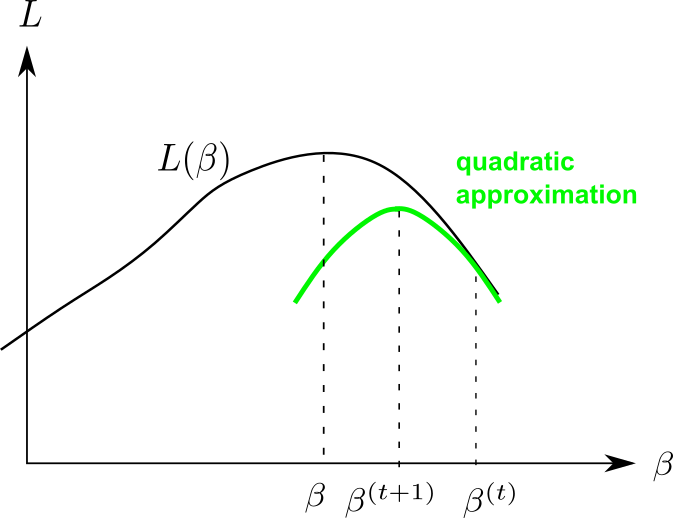
\includegraphics[width=3.5in]
{gen-lin-mod/gen-lin-mod.png}
\caption{One cycle of Newton-Raphson method.}
\label{fig-gml-new-rap}
\end{figure}
